% diag_pipeline: TikZ twin of paper/figures/diag_pipeline.pdf (generated by diag_common.py).
% Coordinates are inches (y up). Needs \usepackage{tikz}. Body font 7 pt.
\definecolor{dgA}{HTML}{F0F0F0}\definecolor{dgB}{HTML}{DCDCDC}\definecolor{dgC}{HTML}{C4C4C4}
\definecolor{dgAtk}{HTML}{F2C9B8}\definecolor{dgHw}{HTML}{E3EEF7}
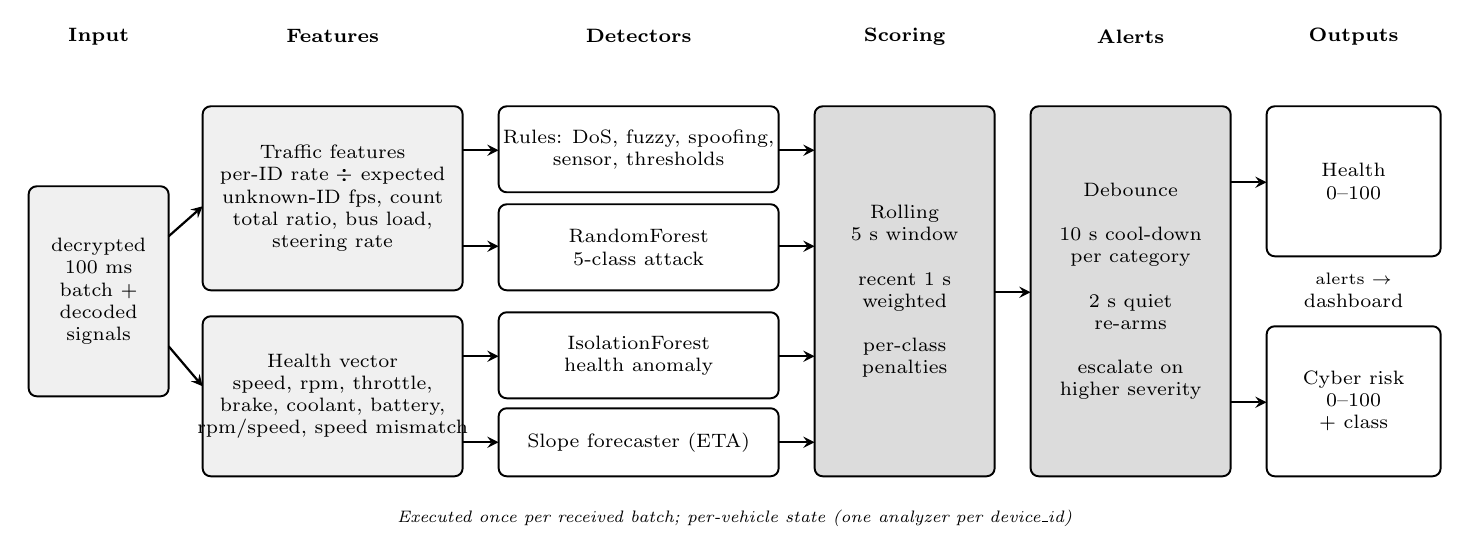
\begin{tikzpicture}[x=1in,y=1in,>=stealth,font=\fontsize{7}{8}\selectfont,line width=0.7pt]
\node[align=center,inner sep=0pt] at (0.400,2.550) {\bfseries \fontsize{7.0}{7.8}\selectfont Input};
\node[align=center,inner sep=0pt] at (1.570,2.550) {\bfseries \fontsize{7.0}{7.8}\selectfont Features};
\node[align=center,inner sep=0pt] at (3.100,2.550) {\bfseries \fontsize{7.0}{7.8}\selectfont Detectors};
\node[align=center,inner sep=0pt] at (4.430,2.550) {\bfseries \fontsize{7.0}{7.8}\selectfont Scoring};
\node[align=center,inner sep=0pt] at (5.560,2.550) {\bfseries \fontsize{7.0}{7.8}\selectfont Alerts};
\node[align=center,inner sep=0pt] at (6.675,2.550) {\bfseries \fontsize{7.0}{7.8}\selectfont Outputs};
\draw[rounded corners=2.9pt,fill=dgA,line width=0.7pt] (0.050,0.750) rectangle (0.750,1.800);
\node[align=center,inner sep=0pt] at (0.400,1.275) {\fontsize{7.0}{7.8}\selectfont decrypted\\ 100 ms\\ batch +\\ decoded\\ signals};
\draw[rounded corners=2.9pt,fill=dgA,line width=0.7pt] (0.920,1.280) rectangle (2.220,2.200);
\node[align=center,inner sep=0pt] at (1.570,1.740) {\fontsize{6.6}{7.4}\selectfont Traffic features\\ per-ID rate ÷ expected\\ unknown-ID fps, count\\ total ratio, bus load,\\ steering rate};
\draw[rounded corners=2.9pt,fill=dgA,line width=0.7pt] (0.920,0.350) rectangle (2.220,1.150);
\node[align=center,inner sep=0pt] at (1.570,0.750) {\fontsize{6.6}{7.4}\selectfont Health vector\\ speed, rpm, throttle,\\ brake, coolant, battery,\\ rpm/speed, speed mismatch};
\draw[->,line width=0.8pt] (0.750,1.550) -- (0.920,1.700);
\draw[->,line width=0.8pt] (0.750,1.000) -- (0.920,0.800);
\draw[rounded corners=2.9pt,fill=white,line width=0.7pt] (2.400,1.770) rectangle (3.800,2.200);
\node[align=center,inner sep=0pt] at (3.100,1.985) {\fontsize{6.8}{7.6}\selectfont Rules: DoS, fuzzy, spoofing,\\ sensor, thresholds};
\draw[rounded corners=2.9pt,fill=white,line width=0.7pt] (2.400,1.280) rectangle (3.800,1.710);
\node[align=center,inner sep=0pt] at (3.100,1.495) {\fontsize{6.8}{7.6}\selectfont RandomForest\\ 5-class attack};
\draw[rounded corners=2.9pt,fill=white,line width=0.7pt] (2.400,0.740) rectangle (3.800,1.170);
\node[align=center,inner sep=0pt] at (3.100,0.955) {\fontsize{6.8}{7.6}\selectfont IsolationForest\\ health anomaly};
\draw[rounded corners=2.9pt,fill=white,line width=0.7pt] (2.400,0.350) rectangle (3.800,0.690);
\node[align=center,inner sep=0pt] at (3.100,0.520) {\fontsize{6.8}{7.6}\selectfont Slope forecaster (ETA)};
\draw[->,line width=0.8pt] (2.220,1.980) -- (2.400,1.980);
\draw[->,line width=0.8pt] (2.220,1.500) -- (2.400,1.500);
\draw[->,line width=0.8pt] (2.220,0.950) -- (2.400,0.950);
\draw[->,line width=0.8pt] (2.220,0.520) -- (2.400,0.520);
\draw[rounded corners=2.9pt,fill=dgB,line width=0.7pt] (3.980,0.350) rectangle (4.880,2.200);
\node[align=center,inner sep=0pt] at (4.430,1.275) {\fontsize{6.8}{7.6}\selectfont Rolling\\ 5 s window\\ \\ recent 1 s\\ weighted\\ \\ per-class\\ penalties};
\draw[->,line width=0.8pt] (3.800,1.980) -- (3.980,1.980);
\draw[->,line width=0.8pt] (3.800,1.500) -- (3.980,1.500);
\draw[->,line width=0.8pt] (3.800,0.950) -- (3.980,0.950);
\draw[->,line width=0.8pt] (3.800,0.520) -- (3.980,0.520);
\draw[rounded corners=2.9pt,fill=dgB,line width=0.7pt] (5.060,0.350) rectangle (6.060,2.200);
\node[align=center,inner sep=0pt] at (5.560,1.275) {\fontsize{6.6}{7.4}\selectfont Debounce\\ \\ 10 s cool-down\\ per category\\ \\ 2 s quiet\\ re-arms\\ \\ escalate on\\ higher severity};
\draw[->,line width=0.8pt] (4.880,1.270) -- (5.060,1.270);
\draw[rounded corners=2.9pt,fill=white,line width=0.7pt] (6.240,1.450) rectangle (7.110,2.200);
\node[align=center,inner sep=0pt] at (6.675,1.825) {\fontsize{6.8}{7.6}\selectfont Health\\ 0--100};
\draw[rounded corners=2.9pt,fill=white,line width=0.7pt] (6.240,0.350) rectangle (7.110,1.100);
\node[align=center,inner sep=0pt] at (6.675,0.725) {\fontsize{6.8}{7.6}\selectfont Cyber risk\\ 0--100\\ + class};
\draw[->,line width=0.8pt] (6.060,1.820) -- (6.240,1.820);
\draw[->,line width=0.8pt] (6.060,0.720) -- (6.240,0.720);
\node[align=center,inner sep=0pt] at (6.675,1.280) {\fontsize{6.5}{7.3}\selectfont alerts $\rightarrow$\\ dashboard};
\node[align=center,inner sep=0pt] at (3.580,0.140) {\itshape \fontsize{6.5}{7.3}\selectfont Executed once per received batch; per-vehicle state (one analyzer per device\_id)};
\end{tikzpicture}
